%! TEX program = xelatex
\documentclass[usenames,dvipsnames]{beamer}
%\usepackage[silent]{fontspec}
\usetheme[sectionpage=none]{metropolis}
%\usepackage{booktabs} 
\usepackage{url}
\def\UrlBreaks{\do\/\do-}
\usepackage{amsfonts, amsmath, lmodern}
\usefonttheme{serif}
\usepackage{algorithm}
\usepackage{algorithmic}

\usepackage{tcolorbox}
\usepackage{xcolor}
\usepackage{csquotes}


%plots
\usepackage{tikz}
\usepackage{pgfplots}
\usepackage{pgfplotstable}
\pgfplotsset{compat=newest}
\usepackage{subcaption}
\usepackage{csvsimple}

\usepackage[backend=biber]{biblatex}
\bibliography{../bibliography/bibliography.bib}
\renewcommand*{\bibfont}{\footnotesize}

%bibliography numbers
%\setbeamertemplate{bibliography item}{\insertbiblabel}

\newcommand{\teamname}{Team Neville Longbottom}




\title{Image Retrieval for Arguments Using Stance-Aware Query Expansion \texorpdfstring{\supercite{kiesel:2021e}}{}}

\author{Bernd Heizmann, Christian Ortlepp, Gustav Lahmann, Max Koch\texorpdfstring{\\$\longrightarrow$ aka \teamname}{aka \teamname}}


\institute{Friedrich-Schiller-Universität Jena}

\date{27.10.2022}

\vfuzz=20pt
\begin{document}
	
	
	\maketitle

	\begin{frame}{Gliederung}
		\tableofcontents
	\end{frame}
	
	\begin{section}{Motivation}
		\begin{frame}{Motivation}
			\begin{itemize}
				\item Bilder spielen eine große Rolle darin den eigenen Standpunkt zu vertreten \& zu verdeutlichen
				\item Beispiele \begin{itemize}
					\item Diagramme
					\item Fotos
					\item Memes
				\end{itemize}
			\item zurzeit gibt es Argumentsuche nur für text (z.B. args.me)
			\end{itemize}
		\end{frame}
	\end{section}
	
	\begin{section}{Methodik}
		\begin{frame}{Methodik}
			\begin{itemize}
				\item[Def:] \textit{"Given a keyword query suggesting an issue or a claim for a topic, retrieve as two ranked lists those and only those images that can assist someone in (1) supporting and (2) attacking it."}
				\item Bewertungskriterien:
					\begin{minipage}[t]{0.5\textwidth}
						\centering
							Topic Relevance \\
							$\uparrow$ \\
							Argumentativeness \\
							$\uparrow$ \\
							Stance relevance
						\end{minipage}
				\item TREC-style Evaluation:
					\begin{itemize}
						\item 12 Personen annotierten 993 Bilder
						\item ersten 10 Ergebnisse für jede Anfrage
						\item Labels: \texttt{pro}, \texttt{contra}, \texttt{both}, \texttt{neither}, \texttt{off topic}
					\end{itemize}
			\end{itemize}
		\end{frame}
	
	\end{section}

	\begin{section}{Ansatz: Stance-Aware Query Expansion}
	\begin{frame}{Grundidee}
		\begin{itemize}
			\item Nutzeranfrage an Google Bildersuche mit Stichworten anreichern, welche einen Standpunkt (Pro oder Contra) vertreten
			\item Auswahl der Stichworte nach drei Methoden:
				\begin{itemize}
					\item (1) Good-Anti
					\item (2) Positive-Negative
					\item (3) Pros-Cons
				\end{itemize}

		\end{itemize}
	\end{frame}

	\begin{frame}{(1) Good-Anti}
		\centering
		\large \textit{Should the federal minimum wage be increased?} \normalsize
		\vspace{2em}
		\begin{tcolorbox}
			\begin{tabular}{l l}
				lemmatisierte Anfrage: \\
				\texttt{increase minimum wage} & \texttt{\color{JungleGreen}good} \\
																			 & \texttt{\color{RubineRed}anti}
			\end{tabular}
		\end{tcolorbox}
\end{frame}
	
\begin{frame}{(2) Positive-Negative}
	\begin{itemize}
		\item Hinzufügen von \enquote{co-occuring} Wörtern (nach Leipzig Corpora Collection's English corpus) aus dem MPQA subjectivity lexicon
		\vspace{1em}
		\begin{tcolorbox}
			\begin{tabular}{l l}
				\texttt{increase minimum wage} & \texttt{\color{RubineRed}poverty} \\
																			 & \texttt{\color{RubineRed}long} \\
																			 & \texttt{\color{RubineRed}little} \\
																			 & \texttt{\color{RubineRed}mean} \\
				\texttt{increase minimum wage} & \texttt{\color{JungleGreen}will} \\
																			 & \texttt{\color{JungleGreen}like} \\
																			 & \texttt{\color{JungleGreen}just} \\
																			 & \texttt{\color{JungleGreen}support} \\
			\end{tabular}
		\end{tcolorbox}
	\end{itemize}
\end{frame}

\begin{frame}[plain]
	\hfill \small \textit{corpora.uni-leipzig.de}
	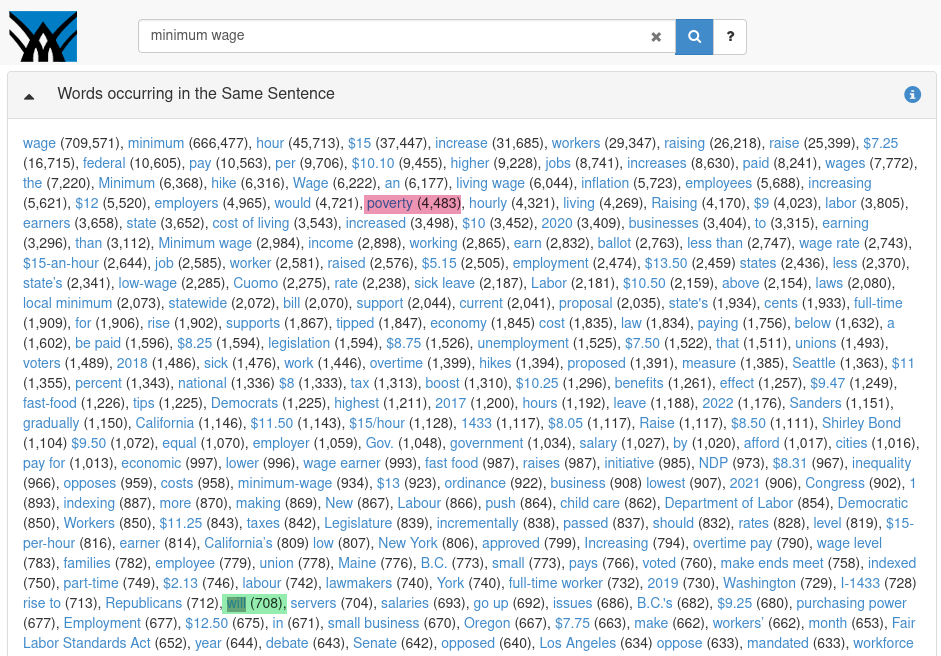
\includegraphics[width=\textwidth]{figures/corpora-minimum-wage.png}
\end{frame}

\begin{frame}{(3) Pros-Cons}
	\begin{itemize}
		\item nutzt args.me um Argumente für pro/con zu finden
		\item ausgenommen \textit{debate.org}
		%TODO diese Wahrscheinlichkeits-Berechnungnen
		\vspace{1em}
		\begin{tcolorbox}
			\begin{tabular}{l l}
				\texttt{increase minimum wage} & \texttt{\color{RubineRed}employment} \\
																			 & \texttt{\color{RubineRed}find} \\
																			 & \texttt{\color{RubineRed}exploitation} \\
																			 & \texttt{\color{RubineRed}unemployment} \\
																			 & \texttt{\color{RubineRed}employ} \\
				\texttt{increase minimum wage} & \texttt{\color{JungleGreen}society} \\
																			 & \texttt{\color{JungleGreen}model} \\
																			 & \texttt{\color{JungleGreen}wage} \\
																			 & \texttt{\color{JungleGreen}woman} \\
																			 & \texttt{\color{JungleGreen}year} \\
			\end{tabular}
		\end{tcolorbox}
	\end{itemize}
\end{frame}
\end{section}
	
	\begin{section}{Ergebnisse}
		\begin{frame}{Ergebnisse}
			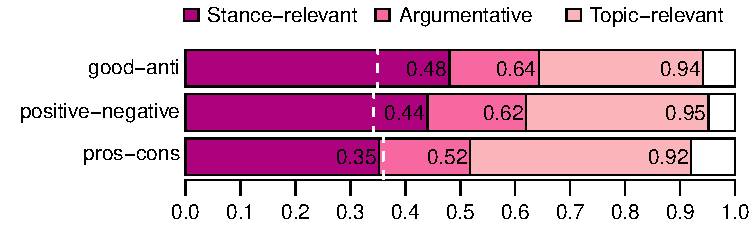
\includegraphics[width=0.9\textwidth]{figures/by-method}
			\begin{itemize}
				\item fast alle (92-95\%) Bilder on-topic
				\item argumentative precision@10: \begin{itemize}
					\item good-anti 0.64
					\item pros-cons 0.52
				\end{itemize}
				\item stance-relevance 16-18 Prozentpunkte niedriger
			\end{itemize}
		\end{frame}
	
	\begin{frame}{Probleme}
		\begin{itemize}
			\item Bilder oft eher illustrierend als argumentativ
			\item teilweise zu viele Bilder von Shopping-Angeboten
			\item einige Standpunkte werden online eher einseitig argumentiert
		\end{itemize}
	\end{frame}
	\end{section}
	
	\begin{frame}[allowframebreaks]{Bibliography}
		\printbibliography
	\end{frame}
	%TODO Bilder?
	%TODO Stichpunkte auf Englisch?
	
\end{document}
